\epigraph{For neural machine translation, it all started from language
modeling.}{Thang Luong.}

Language modeling plays an
indispensable role in ensuring that machine translation systems produce fluent target
sentences and has always been an active area of research.
Despite much effort in improving traditional \ngram{} language models
\cite{rosenfeld2000,srilm,teh2006,irstlm,kenlm,pauls2011,heafield13},
traditional LMs inherently can only handle short
contexts of a few words. Approaches to building \nlmtext{} (\nlms) using
feed-forward networks such as those initiated by \newcite{Bengio2003} and
enhanced by others \cite{Morin2005,Bengio08,MnihHinton2009,MnihTeh2012} have %,Mnih2007
addressed that drawback to model longer contexts.
% worked great compared to traditional \ngram{} language models. 
Still, \nlms{} can only capture fixed-length contexts and is
incapable of handling variable-length sequences, which is the case for sentences.
Recurrent neural networks (RNNs) come in handy as a powerful and expressive
architecture to handle sequential data and have successfully been applied to the
language modeling task \cite{MikolovKBCK10,MikolovKBCK11,mikolovLM}.
By viewing RNNs as generative models \cite{Sutskever11} that can produce texts 
and by pushing another step towards conditioning RNNs on source sentences, recent works
\cite{kal13,sutskever14,cho14} have started a new line of resesarch in machine translation, namely Neural
Machine Translation (NMT). NMT is technically a source-conditioned \nlm{} that
can be trained end-to-end.

%Early success of feed-forward \nlms{} has led to widespread adoption of \nlms{}
%as an additional component in the machine translation pipeline
%such as \cite{schwenk07,vaswani13decode,luong15nlm}, inter alia.
%\cite{Schwenk12continuous,Son:2012:CST,Auli13,devlin14}

%An important part in the machine translation pipeline is the ability to model language
%coherence at the target side. 
%As such, a significant amount of effort in
%improving MT has centered around enhancing language modeling -- more specifically, the need to capture long-range
%dependencies better. We start out with efforts to scale up traditional \ngram{} language models 

In this chapter, we provide background knowledge on two main topics, RNN and NMT.
We first go through the basics of RNNs, explaining how they can be used to model sentences. 
Then, we delve into details of one particular type of RNNs, the Long Short-term Memory, that makes training RNNs easier.
Given RNNs as a building block, we discuss NMT together with tips and tricks for better training and testing NMT.

\section{Recurrent Neural Network}
\label{sec:rnn}
Recurrent Neural Network (RNNs) \cite{elman90} are models that help understand
the temporal aspect as well as build up representations for sequential data
using a dynamic memory structure. At the surface form, an RNN takes as input a sequence of vectors $\x{1},
\x{2}, \ldots, \x{n}$ and processes them one by one. For each
new input $\x{i}$, an RNN updates its memory to produce a hidden state
$\hid{i}$ which one can think of as a representation for the partial sequence
$\x{\overline{1,i}}$. %$\x{1},\ldots, \x{i}$. 
The beauty of RNNs lies in the fact that it can
capture the dynamics of an arbitrarily long sequence without having to increase its modeling
capacity unlike the case of feedforward network which can only model
relationship within a fixed-length sequence. The key secret sauce is in the
recurrence formula of an RNN that defines how its hidden state is updated. At
its simplest form, a ``vanilla'' RNN defines its recurrence function as:
\begin{align}
\hid{t} &= f\paren{\x{t}, \hid{t-1}} \label{e:abstract_rnn}
\end{align}
In the above formula, $f$ is an abstract function that computes a new hidden state given the current input $\x{t}$ and the
previous hidden state $\hid{t-1}$. The starting state $\hid{0}$ is often set to
$\bm{0}$ though it can take any value as we will see later in the context
of NMT decoders. A popular choice of $f$ is provided below with $\sigma$ being a
non-linear function such as $\sigmoid$ or $\tanh$.\footnote{There could also be
an optional bias term in \eq{e:vanilla_rnn}.}
\begin{align}
%\z{t} &= \W{xh}\x{t} + \W{hh}\hid{t-1} \label{e:vanilla_rnn} \\
\hid{t} &= \sigma(\W{xh}\x{t} + \W{hh}\hid{t-1} \label{e:vanilla_rnn}) %\z{t})
\end{align}

At each timestep $t$, an RNN can (optionally) emit an output symbol
$y_t$ which can either be discrete or real-valued. For the discrete scenario,
which is often the case for languages, a probability distribution $\bm{p}$ over a 
set of output classes $Y$ is derived as
follows\footnote{For the real-valued case, we refer readers to mixture density
models \cite{bishop94} which have been applied to RNN training, e.g., for
hand-writing synthesis \cite{graves13c}.}:
\begin{align}
\s{t} &= \W{hy}\hid{t} \label{e:score} \\
\prob{t} &= \softmax(\s{t}) \label{e:prob}
\end{align}
Here, we introduce a new set of weights $\W{hy} \inR{|Y| \times d}$, with $d$ being the dimension of the RNN hidden
state, to compute a score vector $\s{t}$, or {\it logits}, over
different individual classes. Often, with a large output set $Y$, the
matrix-vector multiplication in \eq{e:score} is a major computational
bottleneck in RNNs, which results in several challenges for neural language modeling
and machine translation that we will address in later chapters. 
The $\softmax$ function transforms the score
vector $\s{t}$ into a probability vector $\prob{t}$, which is defined for each specific
element $y \in Y$ as below.
For convenience, we overload our notations to use $\prob{t}(y)$ and $\s{t}(y)$ to refer to entries in
the vectors $\prob{t}$ and $\s{t}$ that correspond to $y$.
\begin{align}
\prob{t}(y) = \frac{\e^{\s{t}(y)}}{\sum_{y' \in Y} \e^{\s{t}(y')}}
\label{e:softmax}
\end{align}

With the above formulas, we have completely defined the RNN weight set $\thetav$
%=\!\{\W{xh}, \W{hh}, \W{hy}\}$, 
which consists of {\it input} connections $\W{xh}$, {\it
recurrent} connections $\W{hh}$, and {\it output}
connections $\W{hy}$. These weights are shared across
timesteps as illustrated in Figure~\ref{f:rnn} \error{Draw a picture on
general RNNs}, which enables
RNNs to handle arbitrarily long sequences.

\begin{figure}[tbh!]
\centering
%\psgrid
\rput(7.1,2.6){{\color{lightblue} $\MB{W_{hh}}$}}
\rput(8.6,1.0){{\color{lightgreen} $\MB{W_{xh}}$}}
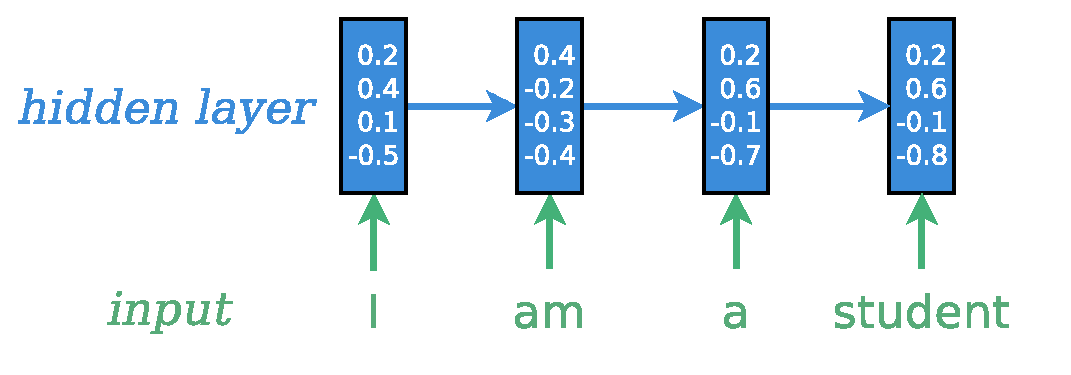
\includegraphics[width=0.6\textwidth, clip=true, trim= 0 0 0 0]{img/rnn.eps} % , angle=-90
\caption[Recurrent neural networks]{{\bf Recurrent neural networks} -- example of a recurrent
neural network that processes a sequence of input words \word{I am a student} to
build up hidden representations as input symbols are consumed. The recurrent
$\MB{W_{hh}}$ and feed-forward $\MB{W_{xh}}$ weights are shared across
timesteps.
} 
\label{f:rnn}
\end{figure}

Next, we discuss the training and testing phases of RNNs from a slightly more
focused angle, the language learning aspect. For more details on RNNs, we refer readers to the following resources
\cite{sutskever12,mikolov12,karpathy15rnn}.

\subsection{Recurrent Language Models}
\label{subsec:rlm}
To apply RNNs to sentences in languages, or generally sequences of discrete symbols, one can
consider one-hot representations $\x{i} \inR{|V|}$, with $V$ being the
vocabulary considered. However, for a large
vocabulary $V$, such a representation choice is problematic as it results in
a large weight matrix $\W{xh}$ and there is no notion of similarity between
words. In practice, low-dimensional dense representations for words, or {\it
word embeddings}, are often used to address these problems. Specifically, an
embedding matrix
$\W{e} \inR{d_e \times |V|}$ is looked up for each word $x_i$ to retrieve a
representation $\x{i} \inR{d_e}$. As a result, a simple RNN applied to language
modeling will generally have $\theta = \{\W{xh}, \W{hh}, \W{hy}, \W{e}\}$ as its
weights as illustrated in Figure~\ref{f:rlm} \error{Draw an RNN with
embedding}.

\begin{figure}[tbh!]
\centering
%\psgrid
\rput(7.1,2.6){{\color{lightblue} $\MB{W_{hh}}$}}
\rput(8.6,1.0){{\color{lightgreen} $\MB{W_{xh}}$}}
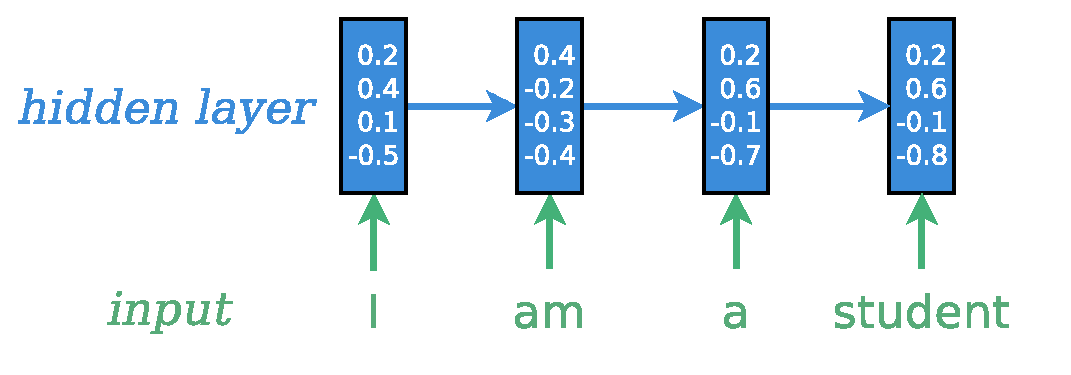
\includegraphics[width=0.6\textwidth, clip=true, trim= 0 0 0 0]{img/rnn.eps} % , angle=-90
\caption[Recurrent language models]{{\bf Recurrent language models} -- example of a recurrent
neural network that processes a sequence of input words \word{I am a student} to
build up hidden representations as input symbols are consumed. The recurrent
$\MB{W_{hh}}$ and feed-forward $\MB{W_{xh}}$ weights are shared across
timesteps.
} 
\label{f:rlm}
\end{figure}

In language modeling (LM), the task is to specify a probability distribution over
sequences of symbols (often, words) so that one can judge if a sequence of
words is more likely or ``fluent'' than another. To accomplish that, an LM decomposes the
probability of a word sequence $y = y_1, \ldots,
y_m$ as:
\begin{align}
p(y) = \prod_{i=1}^m p(y_i | y_{<i}) %\yrange{1}{i-1})
\end{align}
In the above formula, each of the
individual term $p(y_i | y_{<i})$ is the conditional probability of the current
word $y_i$ given previous words $y_{<i}$, also referred as the {\it
context} or the {\it history}. To model these conditional probabilities, traditional \ngram{}
as well as feedforward-based neural language models have to resort to the
Markovian assumption to model only a fixed window of context, i.e., $p(y_i |
y_{i-n+1}, \ldots, y_{i-1})$. An RNN-based language model naturally lends itself to model the full
history as we shall see now.

An RNN-based language model (RNNLM) is a special case of RNNs in which: (a) the input and output
are sequences of discrete words, (b) the output sequence ends %$y=\{y_1, \ldots, y_n$, \eos$\}$ 
with a special symbol \eos{} that marks the boundary, e.g., $y=\{$ ``I'', ``am'', ``a'',
``student'', \eos$\}$, and (c) the input sequence is a
shift-by-1 version of the output sequence with \sos{} as a starting symbol,
e.g., $x=\{$ \sos, ``I'', ``am'', ``a'',
``student''$\}$. We illustrate this in \figref{f:rlm}.

%i.e., $x=\{$
%\sos{}, $y_1, \dots, y_n\}$. In our example, $x=\{$ \sos, ``I'', ``am'', ``a'',
%``student''$\}$, whereas $y=\{$ ``I'', ``am'', ``a'',
%``student'', \eos$\}$
\paragraph{Training}
Given a training dataset of $N$ discrete output sequences $\ytop{1}, \ldots,
\ytop{N}$ with lengths $m_1, \ldots, m_N$ accordingly. The learning objective is
to minimize the negative log-likelihood, or the {\it cross-entropy} loss, of these training examples:
\begin{align}
J(\thetav) &= \sum_{i=1}^{N} -\log p\paren{\ytop{i}} \\ 
&= \sum_{i=1}^{N} \sum_{t=1}^{m_i} -\log p\paren{\ytop{i}_t |
\ytop{i}_{<t}}
\label{e:objective}
\end{align}

RNN learning is often done using mini-batch stochastic gradient descent (SGD) algorithms in
which a small set of training examples, a {\it mini-batch}, is used to compute
the gradients and update weights one at a time. Using mini-batches has
several advantages: (a) the gradients are more reliable and consistent than the
``online'' setting which updates per example, (b) less computation is required to
update the weights unlike the case of full-batch learning which has to process
all examples before updating, and (c) with multiple examples in a mini-batch,
one can turn matrix-vector multiplications such
as those in \eq{e:vanilla_rnn} and \eq{e:score} into matrix-matrix multiplications which can be
deployed efficiently on GPUs. The simplest weight update formula with $\eta$ as
a learning rate is given below:
\begin{align}
\thetav \longleftarrow \thetav - \eta \grad{J(\thetav)} %\fracder{J(\thetav)}{\thetav}
\end{align}

\paragraph{Single-timestep Backpropagation} To compute the gradients for the loss $J(\thetav)$,
we first need to be able to derive the gradients of the per-timestep loss $l_t
=\log \prob{t}(y_t)$ with respect to both the RNN weights
$\{\W{xh}, \W{hh}, \W{hy}\}$ and the inputs $\{\x{t}, \hid{t-1}\}$. We denote
these gradients as $\{d\W{xh}, d\W{hh}, d\W{hy}, d\x{t}, d\hid{t-1}\}$
respectively and define intermediate gradients $d\s{t}, d\hid{t}$ similarly. 
Starting with the loss $l_t$, we employ backpropagation through structures
\cite{goller:ieeenn00} to derive each gradient one by one in the following
order: $l_t \rightarrow \s{t} \rightarrow \{\hid{t}, \W{hy}\} \rightarrow
\{\x{t}, \hid{t-1}, \W{xh}, \W{hh}\}$. To simplify the math, we will utilize
several lemmas and corollaries provided in Appendix~\ref{c:misc}.

First, from \eq{e:softmax}, we have:
\begin{align}
d\s{t} = \fracder{\l_t}{\s{t}} = \parfrac{\s{t}} \paren{\s{t}(y_t) - \log \sum_{y'}
e^{\s{t}(y')}}
\end{align}

Computing per-coordinate gradient $\s{t}(y)$ gives:
\begin{align}
 \parfrac{\s{t}(y)} \paren{\s{t}(y_t) - \log \sum_{y'} e^{\s{t}(y')}} =
  \begin{cases}
   1 - \prob{t}(y_t) & y = y_t \\
   -\prob{t}(y) & y \neq y_t
  \end{cases}
\end{align}

The above gradients can be concisely written in vector form as:
\begin{align}
d\s{t} = \bm{1}_{y_t} - \prob{t}
\end{align}

Here, $\prob{t}$ is the probability distribution defined in \eq{e:prob} and has
been calculated in the forward pass,
so we simply reuse it. $\bm{1}_{y_t}$ is a one-hot vector with 1 at position
$y_t$. 
Applying Corollary~\ref{c:chain_rule}, noting that $\s{t} = \W{hy}\hid{t}$ in
\eq{e:score}, we
arrive at:
\begin{align}
% h_t
d\hid{t} &=  \tp{\W{hy}} \cdot d\s{t} \label{e:grad_ht}\\
% W_hy
d\W{hy} &=  d\s{t} \cdot \tp{\hid{t}} \label{e:grad_Why}
\end{align}

At this point, we have derived part of the backpropation procedure which can be
applied to any hidden unit type, e.g., the aforementioned vanilla RNN or the
LSTM unit that we will describe shortly in the next section. 

{\it Vanilla RNN Backpropagation} \indent 
%For the vanilla RNN formulation in \eq{e:vanilla_rnn}, we further backpropagate
%the loss as follows.
%For simplicity and convenience, one can set the embedding size to be equal to the
%hidden size, so $\W{xh}, \W{hh} \inR{d \times d}$. We can further 
First of all, we can simplify the notation to have $\rnn\!=\![\MB{W_{xh}}
\MB{W_{hh}}]$ and $\z{t}\!=\![\x{t};
\hid{t-1}]$, so the RNN formulation in \eq{e:vanilla_rnn} % \inR{2d}
becomes:
\begin{align}
\MB{h_t} = \sigma \paren{\rnn \z{t}} \label{e:rnn_simplified}
\end{align}

Applying \lemmaref{l:chain_rule}, we have:
\begin{align}
% z_t
d\z{t} &=  \tp{\rnn} \cdot
\paren{\sigma'(\rnn \z{t}) \edot d\hid{t}} \label{e:grad_zt} \\
% T_dx2d 
d\rnn &=  \paren{\sigma'(\rnn \z{t}) \edot d\hid{t}} \cdot \tp{\z{t}} \label{e:grad_rnn}
\end{align}

This is one of the {\it tricks} that we use to better utilize GPUs by creating
larger matrices and vectors, i.e., $\rnn$ and $\z{t}$. From \eq{e:grad_zt} and
\eq{e:grad_rnn}, one can easily extract the following gradients:
(a) $d\x{t}$ -- embedding gradients which we use to sparsely update the embedding weights $\W{e}$, (b) $d\hid{t-1}$
 -- gradients of the previous hidden state, which is needed by the
 backpropagation-through-time algorithm that we will discuss next, and (c) $d\W{xh}$ as well
as $d\W{hh}$ -- the RNN input and recurrent connections.\footnote{One can also
separately derive these gradients as follows:
\begin{align}
% x_t
d\x{t} &=  \tp{\W{xh}} \cdot \paren{\sigma'(\rnn \z{t}) \edot d\hid{t}} \label{e:grad_xt}\\
% h_{t-1}
d\hid{t-1} &=  \tp{\W{hh}} \cdot \paren{\sigma'(\rnn \z{t}) \edot d\hid{t}}\\
% W_xh 
d\W{xh} &=  \paren{\sigma'(\rnn \z{t}) \edot d\hid{t}} \cdot \tp{\x{t}} \\
% W_hh 
d\W{hh} &=  \paren{\sigma'(\rnn \z{t}) \edot d\hid{t}} \cdot \tp{\hid{t-1}} \label{e:grad_Whh}
\end{align}
}

\paragraph{Backpropagation Through Time (BPTT)}
Having defined a single-timestep backpropagation procedure, we are now ready to
go through the BPTT algorithm \cite{Rumelhart:1986:LPT,werbos1990}. Inspired by 
\newcite{sutskever12}, we summarize the BPTT algorithm for RNNs below with the
following remarks: (a) Lines 3, 5, 6, 7 accumulate the gradients of RNN weights
$\{\W{hy}, \W{xh}, \W{hh}, \W{e}\}$ over time; (b) In line 7, $d\x{t}$ refers to
gradients of words participating in the current mini-batch which we use to
sparsely update $\W{e}$;\footnote{In multi-layer
RNNs, $d\x{t}$ is used to send gradients down to the below layers.} and (c) Line
4 accumulates gradients for the current hidden state $\hid{t}$ by considering two paths,
a ``vertical'' one from  the current loss at time $t$ and a ``recurrent'' one from the timestep
$t+1$ which was set in Line 8 earlier.

\begin{algorithm}
\For{$t=T \rightarrow 1$}
{
\tcp{Output backprop}
% d_s
$d\s{t} \leftarrow \bm{1}_{y_t} - \prob{t}$

% W_hy
$d\W{hy} \leftarrow d\W{hy} + d\s{t} \cdot \tp{\hid{t}}$

% h_t
$d\hid{t} \leftarrow d\hid{t} + \tp{\W{hy}} \cdot d\s{t}$

\tcp{RNN backprop}
% W_xh 
$d\W{xh} \leftarrow d\W{xh} + \paren{\sigma'(\rnn \z{t}) \edot d\hid{t}} \cdot \tp{\x{t}}$

% W_hh 
$d\W{hh} \leftarrow d\W{hh} + \paren{\sigma'(\rnn \z{t}) \edot d\hid{t}} \cdot \tp{\hid{t-1}}$

\tcp{Input backprop}
% x_t
$d\x{t} \leftarrow \tp{\W{xh}} \cdot \paren{\sigma'(\rnn \z{t}) \edot d\hid{t}}$

% h_{t-1}
$d\hid{t-1} \leftarrow \tp{\W{hh}} \cdot \paren{\sigma'(\rnn \z{t}) \edot d\hid{t}}$
}
\caption{BPTT algorithm for ``vanilla'' RNNs}
\end{algorithm}

\subsection{Better Training RNNs}
Even though computing RNN gradients is straightforward once 
the BPTT algorithm has been plotted out, training is inherently difficult due to the nonlinear
iterative nature of RNNs. Among all reasons, 
the two classic problems of RNNs that often arise when dealing with very long sequences are the {\it
exploding} and {\it vanishing} gradients as
described by \newcite{Bengio-trnn94}. In short, exploding gradients refers to the
phenomenon that the gradients become exponentially large as we backpropagate
over time, making learning unstable. Vanishing gradients, on the
other hand, is the opposite problem when the gradients go exponentially fast
towards zero, turning BPTT into truncated BPTT that is unable to capture long-range
dependencies in sequences. 

Let us try to explain the aforementioned problems informally and 
refer readers to more rigorous and in-depth analyses in \cite{Bengio-trnn94,lstm97,MartensS11,pascanu13}.
The main cause of these two problems all lies in Line 8 of the BPTT
algorithm which can be rewritten as
$d\hid{t-1} = \tp{\W{hh}} \cdot \diag\paren{\sigma'(\rnn \z{t})} \cdot
d\hid{t}$ (see \lemmaref{l:diag_mul}). We can try to understand the behavior of RNNs over time by assuming
for a moment that there is no contribution from intermediate losses, i.e., Line 4
is ``ignored''. Given such an assumption, a signal backpropagated from the current hidden state over K
steps will become 
$d\hid{t-K} = \prod_{i=1}^{K} \paren{\tp{\W{hh}} \cdot \diag\paren{\sigma'(\rnn
\z{t-i+1})}} \cdot
d\hid{t}$. Assuming that the non-linear function $\sigma$ is bounded, e.g.,
$\sigm$ and $\tanh$, and behaves ``nicely'', what we need to deal with now is
the multiplication of the recurrent matrix over time.
This leads to the fact that the behavior of RNNs is often governed by the characteristics of the recurrent matrix
$\W{hh}$ and most analyses examine in terms of the largest eigen value of
$\W{hh}$ as well as the norms of these signals. Roughly speaking, if the largest eigen value
is large enough, exploding gradients will be likely to happen. On the contrary,
if the largest eigen value is below a certain threshold, vanishing gradients
will occur as clearly explained by \newcite{pascanu13}.

\paragraph{Gradient Clipping} In practice, it is generally easy to cope with the exploding gradient problem by
applying different forms of gradient clipping. The first approach was proposed by
\newcite{mikolov12} through the form of temporal {\it element-wise} clipping. At
each timestep during backpropagation, any elements of $d\bm{h}$ that are greater
than a positive threshold $\tau$ or smaller than -$\tau$ will be set
to $\tau$ or -$\tau$ respectively. One can also perform gradient {\it norm}
clipping as suggested by \newcite{pascanu13}. The idea is simple: given a final
gradient vector $\bm{g}$ computed per mini-batch, if its norm
$||\bm{g}||$ is greater than a threshold
$\tau$, then we will use the following scaled gradient $\frac{\tau}{||\bm{g}||} \bm{g}$
instead. The latter approach has been widely used in many systems nowadays and
can also be used in conjunction with the former. We take the combined approach
in our implementations described later in this thesis. 

\paragraph{Long Short-Term Memory}
The vanishing gradient problem, on the other hand, is more challenging to
tackle. There have been many proposed approaches to alleviate the problem such
as skip connections \cite{waibel90,lin96}, hierarchical
architectures \cite{el96}, leaky integrators \cite{Jaeger2007}, second-order
methods \cite{MartensS11}, and
regularization \cite{pascanu13}, to name a few; also, see \cite{bengio13} for a
comparison of some of these techniques. Among all, Long Short-term
Memory (LSTM), invented by \newcite{lstm97}, appears to be one of the most
widely adopted solutions to the vanishing gradient problem.
Graves and colleagues deserve credit for popularizing LSTM through a series of
work \cite{graves05,graves09,graves13c}. 
The key idea of LSTM
is to augment RNNs with linear {\it memory} units that allow the gradient to
flow smoothly through time. In addition, there are gating units that control how
much an RNN wants to reuse memory ({\it forget} gates), receive input signal ({\it
input} gates), and extract information ({\it output} gates) at each timestep.
There are many implementation instances of LSTM, differing in terms of
whether and which biases are used, how gates are built, etc; however, it turns
out that these different choices do not matter much for most cases
\cite{jozefowicz15,greff15}. As such, in this section and through out this
thesis, we will stick to the formulation described in \cite{zaremba14}.

Instead of jumping directly into the detailed formulation, let us provide intuitions
on how to gradually build up an LSTM architecture. First, we can construct a
simple memory unit as follows:
\begin{align}
\mem{t} &= \mem{t-1} + \sigma\paren{\W{xh}\x{t} + \W{hh}\hid{t-1}}
\label{e:simple_mem}) \\
\hid{t} &= \mem{t}
\end{align}

This architecture can be viewed as a form of ``leaky'' integration 
mentioned in \cite{sutskever12,bengio13} since it is equivalent to $\hid{t} =
\hid{t-1} + \sigma(\W{xh}\x{t} + \W{hh}\hid{t-1})$. Training this
network over long sequences is easy since among the exponentially many backpropagation
paths, there is exactly one path that goes through all the memory units
$\mem{i}$ ($i=\overline{1,T}$) and is
guaranteed to not vanish since $d\mem{t} = d\mem{t-1}$ along that path. 

Such architecture, however, does not account for the fact that certain inputs,
e.g., function words or punctuations,
are, sometimes, not relevant to the task at hand and should be downweighted.
Occasionally, we might also want
to reset the memory, e.g., at the beginning of each sentence in a
paragraph. To add more flexibility and power to this architecture, the LSTM adds
forget, input, and output gates as follows:
\begin{align}
\mem{t} &= \fg \edot \mem{t-1} + \ig \edot \sigma\paren{\W{xh}\x{t} +
\W{hh}\hid{t-1}} \\
\hid{t} &= \og \edot \sigma\paren{\mem{t}} \label{e:lstm_output})
\end{align}
We note that, in \eq{e:lstm_output}, 
the memory cell $\mem{t}$ is passed through a nonlinear function $\sigma$ before the output
gate $\og$ is used to extract relevant information in the hope for better
information retrieval.
%or the cell 
%before extracting information for $\hid{t}$ using the output gate $\og$,
%we introduce some non-linearity through $\sigma$ to better retrieve information
%from the memory or the cell $\mem{t}$. 
As an evidence, \newcite{greff15} have
shown that such a output nonlinearity is critical to the performance of an LSTM. Moving on, to ensure that the
gates are adaptive, we build them from the information given by the current
input $\x{t}$ and the previous hidden state $\hid{t-1}$. We also want the gates to be in $[0, 1]$,
so $\sigm$ will be used. All
of these desiderata lead to the below LSTM formulation described in
\cite{zaremba14} in which $\sigma$ is chosen to be $\tanh$:
\begin{align}
\begin{pmatrix}
\ig \\
\fg \\
\og \\
\hg
\end{pmatrix}
&= 
\begin{pmatrix}
\sigm \\
\sigm \\
\sigm \\
\tanh
\end{pmatrix}
\begin{bmatrix}
\W{xi} \W{hi} \\
\W{xf} \W{hf} \\
\W{xo} \W{ho} \\
\W{xh} \W{hh}
\end{bmatrix}
\begin{bmatrix}
  \x{t} \\
  \hid{t-1}
\end{bmatrix} \label{e:lstm_detailed}\\
\mem{t} &= \fg \edot \mem{t-1} + \ig \edot \hg \label{e:lstm_cell}\\
\hid{t} &= \og \edot \tanh(\mem{t}) \label{e:lstm_detailed_output}
\end{align}

%In similar spirit as \eq{e:rnn_simplified}, we can be GPU-efficient with
%equations later, we can rewrite \eq{e:lstm_detailed} as:
Following the same spirit as \eq{e:rnn_simplified}, we can be GPU-efficient with
\eq{e:lstm_detailed} since the 8 different submatrices is grouped into a single big matrix,
which we call $\lstm$. Let $\z{t}\!=\![\x{t}; \hid{t-1}]$, what we do is
first multiply $\lstm \z{t}$ and then apply different non-linear functions to
corresponding parts of the output. For the ease of deriving backpropagation
equations later, we can rewrite \eq{e:lstm_detailed} as:
\begin{align}
\ut &= g(\lstm \z{t}) \label{e:lstm_notation} \\
&= g(\xparam\x{t} + \hparam\hid{t-1})
\label{e:lstm simplified}
\end{align}
Here, $g$ is a non-linear function applied element-wise and we define $g$ loosely in the sense that it uses $\tanh$ only for the vector part corresponding to $\hg$ and $\sigm$ for the rest.


%\begin{align}
%\label{e:lstm simplified}
%\begin{pmatrix}
%\ig \\
%\fg \\
%\og \\
%\hg
%\end{pmatrix}
%&= 
%\begin{pmatrix}
%\sigm \paren{\iparam \z{t}} \\
%\sigm \paren{\fparam \z{t}} \\
%\sigm \paren{\oparam \z{t}} \\
%\tanh \paren{\hparam \z{t}}
%\end{pmatrix}
%\end{align}
%Note that $\hparam\!=\![\MB{W_{xh}} \MB{W_{hh}}]$ is the same as $\rnn$ in
%\eq{e:rnn_simplified}; we define $\iparam, \fparam, \oparam$ similarly for the
%input, forget, and output gates.

\paragraph{LSTM Training}
In the LSTM training pipeline, there are many components that are exactly the
same or very similar to RNN training. We will now highlight some key
differences. First of all, LSTM extends the recurrence function to have not just
the hidden states but also the memory cells as both inputs and outputs. The
definition is as below:
\begin{align}
\paren{\hid{t}, \mem{t}} &= f\paren{\x{t}, \hid{t-1}, \mem{t-1}}
\label{e:abstract_lstm}
\end{align}
In our case, the abstract function $f$ is implemented by
Eq.~\ref{e:lstm_detailed}-\ref{e:lstm_detailed_output}. Once $\hid{t}$ is
computed, the prediction process is the same as that of RNNs which is given by
Eq.~\ref{e:score}-\ref{e:softmax}. The training objective in \eq{e:objective}
remains unchanged as well.

\paragraph{LSTM Backpropagation}
Since the prediction procedure is the same, LSTM backpropagation pipeline mimics
that of RNNs up to \eq{e:grad_ht} and \eq{e:grad_Why}, which computes $d\hid{t}$
and $d\W{hy}$ respectively.

Given $d\hid{t}$, we now work backwark to derive other gradients. First,
starting from \eq{e:lstm_detailed_output} and by applying
\lemmaref{l:edot_der}, we have:
\begin{align}                        
d\og = \tanh(\mem{t}) \edot d\hid{t} \\
d\mem{t} = \tanh'(\bm{\mem{t}}) \edot \bm{\og} \edot d\hid{t} 
\end{align} 

Before backpropagating \eq{e:lstm_cell}, once must {\it remember} to update $d\mem{t}$ with the gradient sent back from $\mem{t+1}$, which is accomplished by Lines~6 and 10 of Algorithm~\ref{a:lstm}. Given the updated $d\mem{t}$, we apply Corollary~\ref{c:edot_der} to derive: 
\begin{align}                        
d\fg = \mem{t-1} \edot d\mem{t} \\
d\mem{t-1} = \fg \edot d\mem{t} \\
d\ig = \hg \edot d\mem{t} \\
d\hg = \ig \edot d\mem{t}
\end{align} 

%For \eq{e:lstm simplified}, by applying \lemmaref{l:chain_rule} repeatedly for $\ig, \fg, \og, \hg$, we arrive at:
%\begin{align}
%\der{h} = \tp{\bm{W}} \cdot \paren{f'(\bm{Wh}) \edot \der{v}}
%\\
%\der{W} = \paren{f'(\bm{Wh}) \edot \der{v}} \cdot \tp{\bm{h}} 
%\end{align}

Let $d\ut = [d\ig; d\fg; d\og; d\hg]$ (vertical concatenation), we are now ready to backpropagate through \eq{e:lstm simplified}. In a similar manner as RNNs, Eq.~\ref{e:grad_xt}-\ref{e:grad_Whh}, we arrive at:
\begin{align}
% x_t
d\x{t} &=  \tp{\xparam} \cdot \paren{g'(\lstm \z{t}) \edot d\ut}\\
% h_{t-1}
d\hid{t-1} &=  \tp{\hparam} \cdot \paren{g'(\lstm \z{t}) \edot d\ut}\\
% T_x 
d\xparam &=  \paren{g'(\lstm \z{t}) \edot d\ut} \cdot \tp{\x{t}} \\
% T_h 
d\hparam &=  \paren{g'(\lstm \z{t}) \edot d\ut} \cdot \tp{\hid{t-1}}
\end{align}

All of these gradients can now be put together in the below BPTT algorithm for LSTM:
\begin{algorithm}
\label{a:lstm}
\For{$t=T \rightarrow 1$}
{
\tcp{Output backprop}
% d_s
$d\s{t} \leftarrow \bm{1}_{y_t} - \prob{t}$

% W_hy
$d\W{hy} \leftarrow d\W{hy} + d\s{t} \cdot \tp{\hid{t}}$

% h_t
$d\hid{t} \leftarrow d\hid{t} + \tp{\W{hy}} \cdot d\s{t}$

\tcp{LSTM backprop}
% og
$d\og \leftarrow \tanh(\mem{t}) \edot d\hid{t}$

% ct
$d\mem{t} \leftarrow d\mem{t} + \tanh'(\bm{\mem{t}}) \edot \bm{\og} \edot d\hid{t}$ \tcp*{Already included $d\mem{t+1}$}

% ft
$d\fg \leftarrow \mem{t-1} \edot d\mem{t}$

% it
$d\ig \leftarrow \hg \edot d\mem{t}$

% hhat_t
$d\hg \leftarrow \ig \edot d\mem{t}$

% reset, c{t-1}
$d\mem{t} \leftarrow \fg \edot d\mem{t}$ \tcp*{Compute $d\mem{t-1}$}

$d\ut = [d\ig; d\fg; d\og; d\hg]$

% T_x 
$d\xparam \leftarrow \paren{g'(\lstm \z{t}) \edot d\ut} \cdot \tp{\x{t}}$

% T_h 
$d\hparam \leftarrow  \paren{g'(\lstm \z{t}) \edot d\ut} \cdot \tp{\hid{t-1}}$

\tcp{Input backprop}
% x_t
$d\x{t} \leftarrow  \tp{\xparam} \cdot \paren{g'(\lstm \z{t}) \edot d\ut}$

% h_{t-1}
$d\hid{t-1} \leftarrow  \tp{\hparam} \cdot \paren{g'(\lstm \z{t}) \edot d\ut}$
}
\caption{BPTT algorithm for LSTM}
\label{a:lstm_bptt}
\end{algorithm}

\section{Neural Machine Translation}
Having introduced recurrent language models, one can simply think of
neural machine translation (NMT) as a recurrent language model that conditions
on the source sentence. More formally, NMT aims to directly model the
conditional probability $p(\tgt{}|\src{})$ of translating
a source sentence, $\src{1},\ldots,\src{n}$, to a target sentence, $\tgt{1},\ldots,\tgt{m}$.
It accomplishes this goal through an {\it encoder-decoder} or {\it
sequence-to-sequence} framework
\cite{kal13,sutskever14,cho14}. The {\it encoder} computes a representation $\MB{s}$
for each source sentence. Based on that source representation,
the {\it decoder} generates a translation, one target word at a time, and hence,
decomposes the log conditional probability as:
\begin{equation}
\log p(\tgt{}|\src{}) = \sum_{t=1}^m \nolimits \log
p\paren{\tgt{t}|\tgt{<t},\MB{s}}
\label{e:s2s}
\end{equation}

NMT models vary in terms of the exact architectures to use.
A natural choice for sequential data is the recurrent
neural network (RNN), used by most of the recent NMT work and for both the
encoder and decoder.
RNN models, however, differ in terms of: (a) {\it directionality} -- unidirectional
or bidirectional; (b) {\it depth} -- single or deep multi-layer; and (c) {\it
type} -- often either a vanilla, an LSTM 
\cite{lstm97}, or a gated recurrent unit (GRU) \cite{cho14}.
In general, for the encoder, almost any architecture can be used since we have
fully observed the source sentence. 
For example, \newcite{kal13} used a convolutional neural network for encoding the source.
Choices on the decoder side are more limited since we need to be able
to generate a translation. At the time of this thesis, the most popular choice is a
unidirectional RNN, which simplifies the beam-search decoding algorithm by
producing translations from left to right.

\begin{figure}[tbh!]
\centering
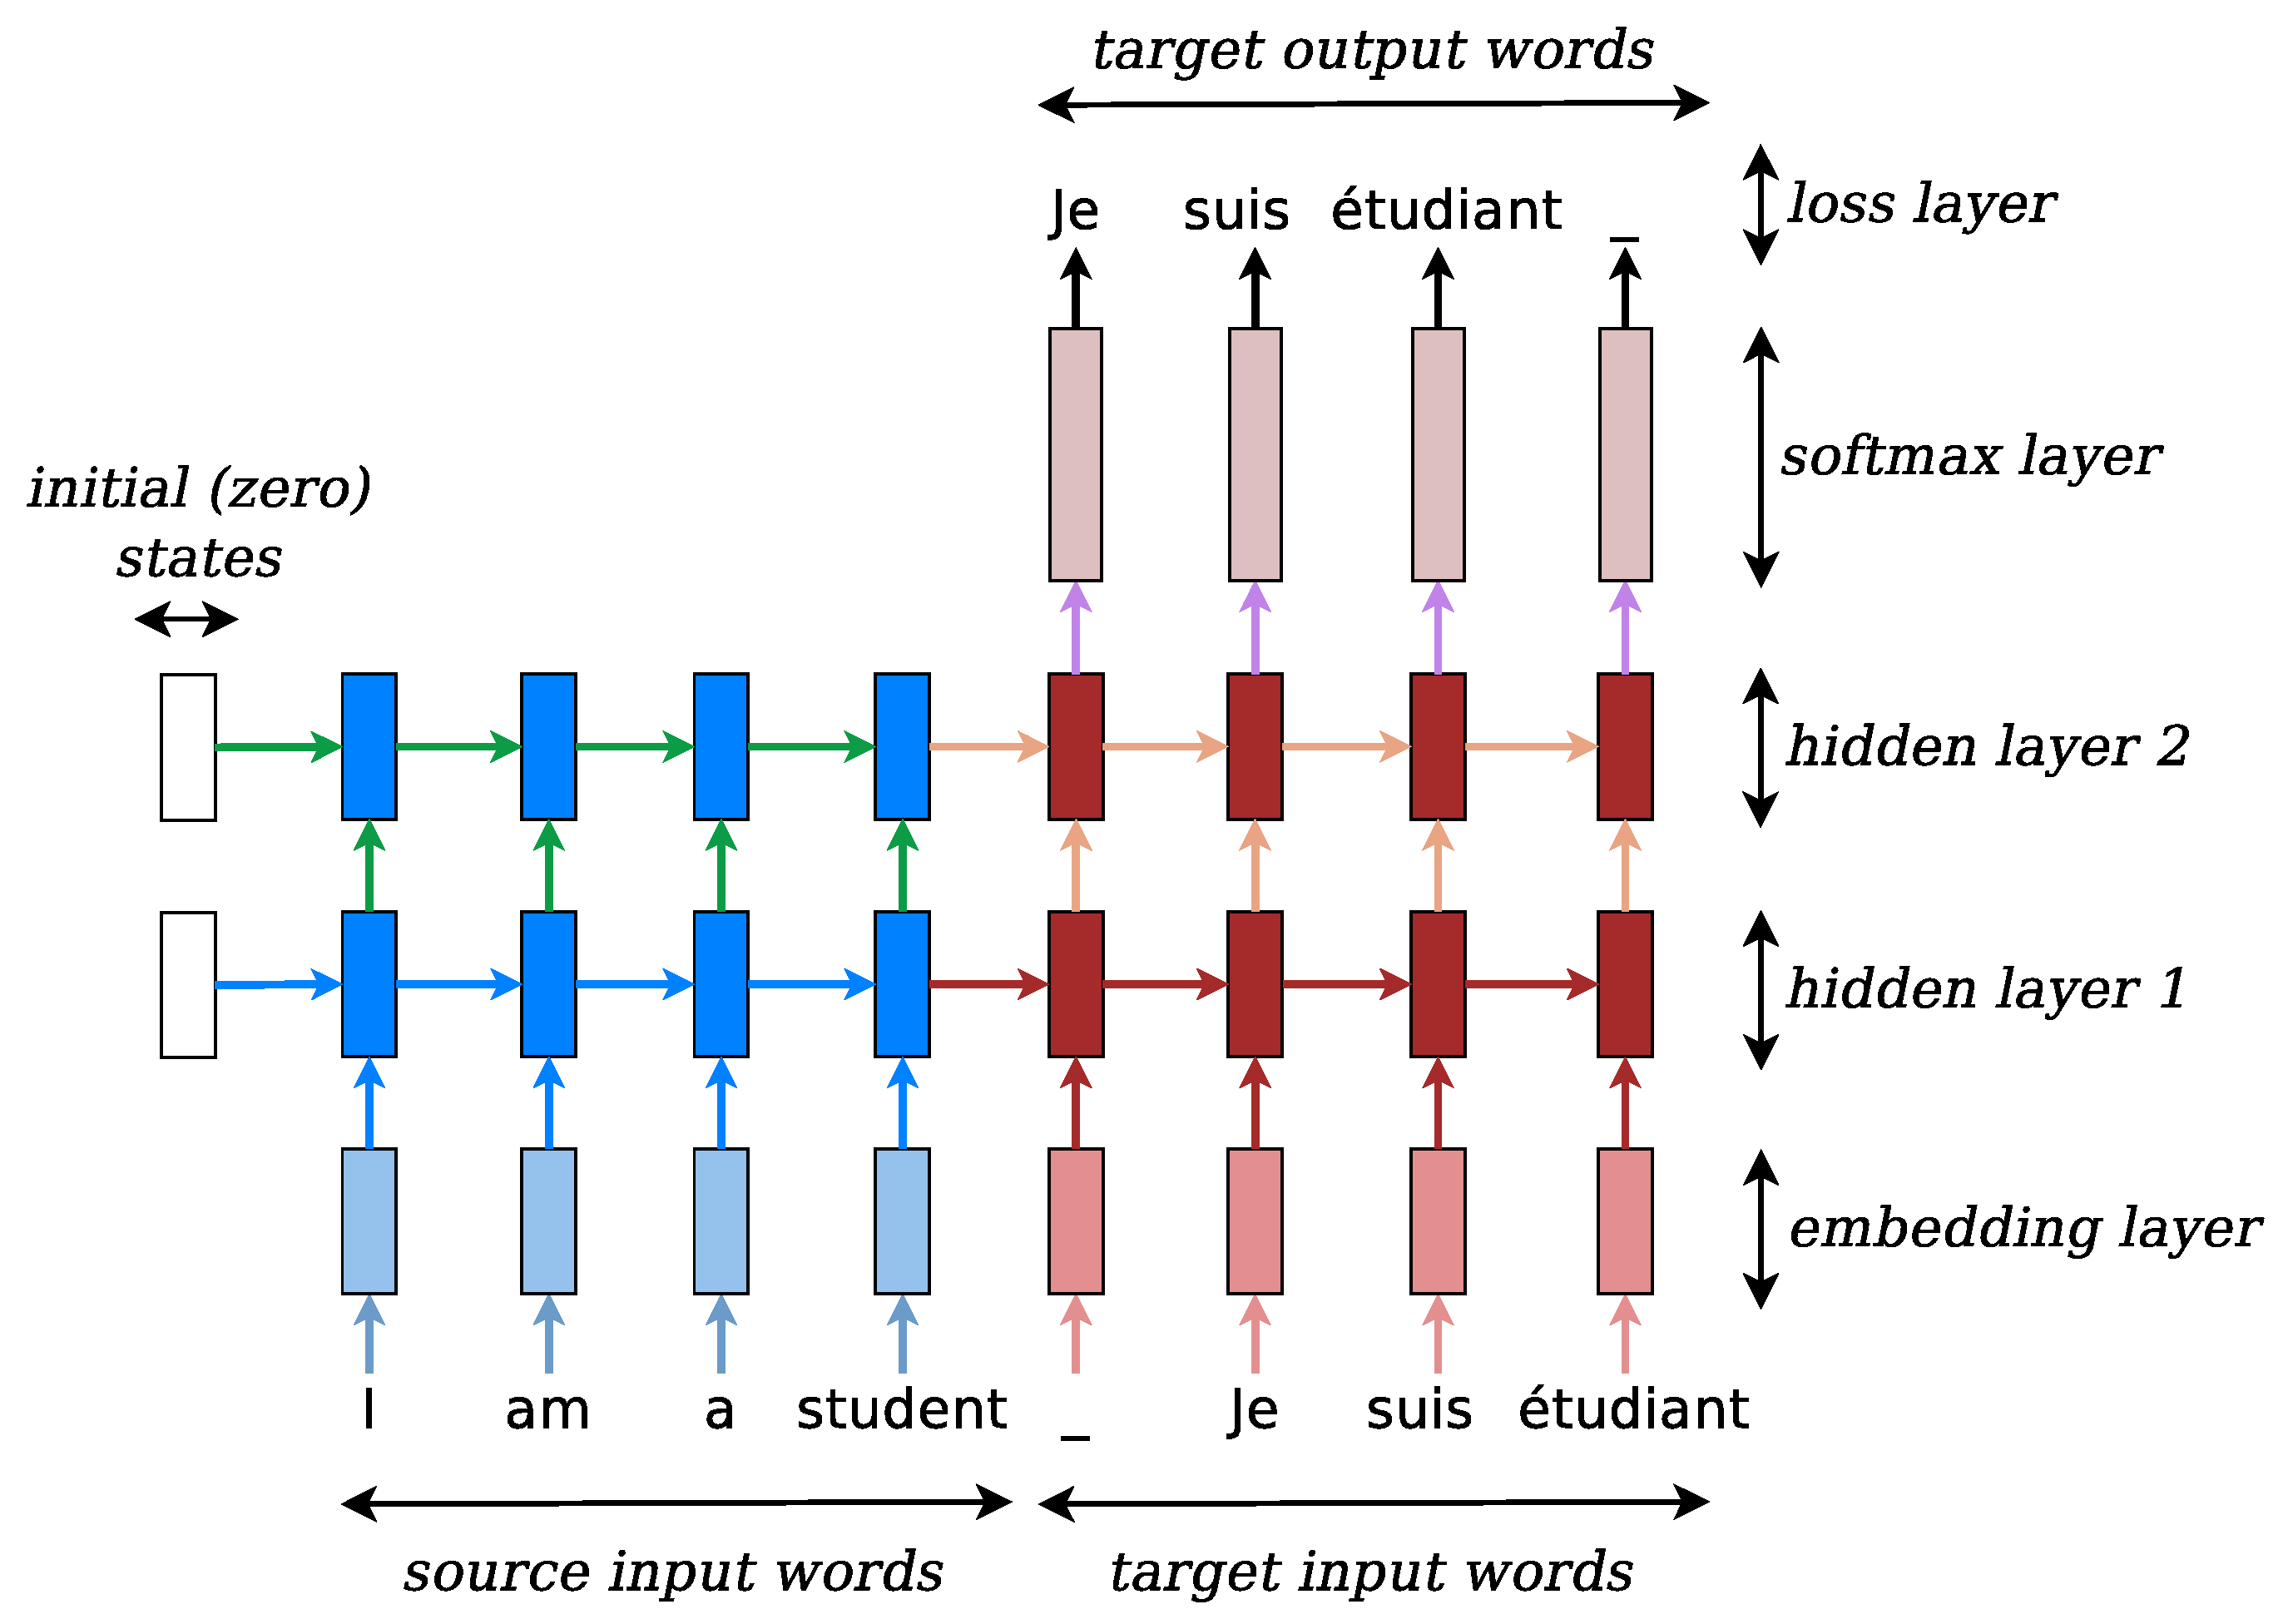
\includegraphics[width=0.8\textwidth, clip=true, trim= 0 0 0
0]{img/nmt_very_details.eps} % , angle=-90
\caption[Neural machine translation]{{\bf Neural machine translation} -- example of a deep recurrent
architecture proposed by \newcite{sutskever14} for
translating a source sentence \word{I am a student} into a target sentence
\word{Je suis \'{e}tudiant}. Here, \word{\texttt{\_}} marks the end of a sentence.
} 
\label{f:nmt_details}
\end{figure}

In this thesis, all our NMT models are deep multi-layer RNNs which are 
unidirectional and have LSTM as the recurrent unit. We show an example of
such model in Figure~\ref{f:nmt_details} though it should be easy to extend to
other RNN architectures. In this example, we train our model to translate a source sentence
\word{I am a student} into a target one \word{Je suis \'{e}tudiant}.
At a high level, our NMT models consist of two recurrent language models as
described in \secref{subsec:rlm}: the {\it encoder} RNN simply consumes the input
source words without making any prediction; the {\it decoder}, on the other
hand, processes
the target sentence while predicting the next words. 

In more detail, at the bottom layer, the encoder and decoder RNNs receive as
{\it input} the following: first,
the source sentence, then a boundary marker \word{\_} which indicates the
transition from the encoding to the decoding mode, and the target sentence. 
Given these discrete words, the model looks up the source and target
embeddings to retrieve the corresponding word representations.
For this {\it embedding layer} to work, a vocabulary is chosen for each language, and
often the top $V$ frequent words are selected.
%Thus, every word in the source or target vocabulary can be represented by a one-hot vector of length $V$.
%The source input sentence and target input sentence, represented as a sequence
%of one-hot vectors, are transformed into a sequence of word embeddings by the
%\emph{embedding} weights. 
These embedding weights, one set per language, are learned during training.
While one can choose to initialize embedding weights with pretrained word
representations, such as word2vec \cite{mikolov13nips} and Glove
\cite{pennington2014}, we found, in this thesis, that these
embeddings can be initialized randomly and learned from scratch given large training datasets.

%, are different for the source words and the target words.
%The word embeddings and all hidden layers are vectors of length $n$ (a chosen hyperparameter).

Once retrieved, the word embeddings are then fed as input into the main network, which consists
of two multi-layer RNNs `stuck together' --- an encoder for the source
language and a decoder for the target language. 
The encoder RNN uses zero vectors as its starting states. The decoder, on the
other hand, needs to have access to the source information, so one simple way to
achieve that is to
initialize it with the last hidden state of the encoder.\footnote{This is not the only way to initialize the decoder,
e.g., \newcite{cho14} connect the last encoder state to every timesteps in the
decoder.} In Figure~\ref{f:nmt_details}, we pass  
the hidden state at the source word \word{student} to the decoder side.
The \emph{feed-forward} (vertical) weights connect
the hidden unit from the layer below to the upper one; whereas, the
\emph{recurrent} (horizontal) weights transfer the history knowlege from the previous
timestep to the next one.
Often, we use different weights across the encoder and decoder as well as
across different layers; in the current example, we have 4 different LSTM
weight sets $\lstm$, detailed in \eq{e:lstm_notation}, over $\{\text{encoder,
decoder}\} \times \{1^{\text{st}}, 2^{\text{nd}} \text{ layer}\}$.
%The hidden state at the top layer of the decoder is fed through an
%\textit{attention} layer, which guides the translation by `paying attention' to relevant parts of the source sentence; 
%for more information see \cite{bahdanau2014neural} or Section 3 of \cite{luong2015effective}.
Finally, for each target word, the hidden state at the top layer is transformed by the
\emph{softmax} weights into a probability distribution over the target
vocabulary of size $V$ according to \eq{e:score} and \eq{e:prob}. 

\paragraph{Training}
Training neural machine translation is similar to training a recurrent
language model that we have discussed in \secref{sec:rnn} except that we need to
handle the conditioning part on source sentences.
The training objective for NMT is formulated as:
\begin{equation}
J = \sum_{(\src{},\tgt{}) \in \mathbb{D}} \nolimits -\log p(\tgt{}|\src{})
\label{e:j_t}
\end{equation}
Here, $\mathbb{D}$ refers to our parallel training corpus of source and target
sentence pairs $(x, y)$. Given the aforementioned NMT architecture,
computing the NMT loss for $(x, y)$ during the {\it forward} pass is
almost the same as how we compute the regular RNN loss on just $y$.
The only difference is that we have to first compute representations for the source
sentence $x$ to initialize the decoder RNN instead of just starting
from zero states. For the {\it backpropagation} phase, computing gradients for
the decoder is the same as what we have described in
Algorithm~\ref{a:lstm_bptt} for regular RNNs. The last hidden-state gradient
from the decoder is
passed back to the encoder. We then continue backpropating through the encoder
in a similar fashion as that of the decoder but without any prediction losses.

More concretely, we present in
\algo{a:nmt_forward} details in the forward pass of an NMT model which uses
a deep multi-layer LSTM architecture. Since the encoder and decoder share
many operations in common, we combine both the source sentence $x$ with length
$m_x$ and the target sentence $y$ with length $m_y$ together to form an input
sequence $s$ as shown in Line 1, which also includes the end-of-sentence marker
\word{\_}. We first start with the encoder parameters (Line~2-3) as well as zero
states and memories (Line~4). The algorithm switches to the decoder mode at time
$m_x + 1$ (Line~6). The encoder and decoder share the same LSTM codebase
(Line~10-14). We first look up the corresponding embeddings for the input
$s_t$; then build up hidden states and memories from the bottom layer to the top
one (the $L^{\text{th}}$ layer). The hidden state computed at one layer is used
as input to the upper one according to Line~13. \texttt{LSTM} in Line~12 refers
to the entire formulation in
Eq~(\ref{e:lstm_detailed}-\ref{e:lstm_detailed_output}), which one can easily
replace with other hidden units such as RNN and GRU. Lastly, on the decoder
side, the top hidden state is used to predict the next symbol $s_{t+1}$
(Line~15-17).

\begin{algorithm}
$s \rightarrow [x, \text{\_}, y, \text{\_}]$ \tcp*{Length of $s$ is $m_x + 1 +
m_y + 1$}
$\W{e} \leftarrow \W{e}^{\text{encoder}}$ \tcp*{Encoder embeddings}
$\lstm \leftarrow \lstm^{\text{encoder}}$ \tcp*{Encoder LSTMs} %multi-layer 
$\hid{0}, \mem{0} \leftarrow \bm{0}, \bm{0}$ \tcp*{Starting states and memories}
% Multi-layer 
%\For{$l=1 \rightarrow L$}{
%$\hid{0}^{(l)}, \mem{0}^{(l)} \leftarrow \bm{0}, \bm{0}$ \tcp*{Starting states and
%memories}
%}
\For{$t=1 \rightarrow (m_x + 1 + m_y)$}
{

\tcp{Decoder transition}
\If{$t == (m_x + 1)$}{
    $\W{e} \leftarrow \W{e}^{\text{decoder}}$ \; % \tcp{Decoder embeddings}
    $\lstm \leftarrow \lstm^{\text{decoder}}$ \; % \tcp{Decoder multi-layer LSTMs}
}

\tcp{Multi-layer LSTM}
% x_t
$\x{t} = \text{LookUp}(s_t, \W{e})$ \;
\For{$l=1 \rightarrow L$} {
    $\hid{t}^{(l)}, \mem{t}^{(l)}= \text{\texttt{LSTM}}\paren{\hid{t-1}^{(l)},
    \mem{t-1}^{(l)}, \x{t}, \lstm^{(l)}}$ \tcp*{LSTM hidden unit}
    $\x{t} = \hid{t}^{(l)}$ \;
}

\tcp{Target-side prediction}
\If{$t \geq (m_x + 1)$}{
    $\text{\texttt{Predict}}(s_{t+1}, \hid{t}^{(L)},\W{hy})$ \;
}
}


mention bucketing and batching




\caption{NMT training algorithm -- {\it forward} pass.}
\label{a:nmt_forward}
\end{algorithm}

\subsection{Testing}

mention beam-search, ensemble

\begin{figure}[tbh!]
\centering
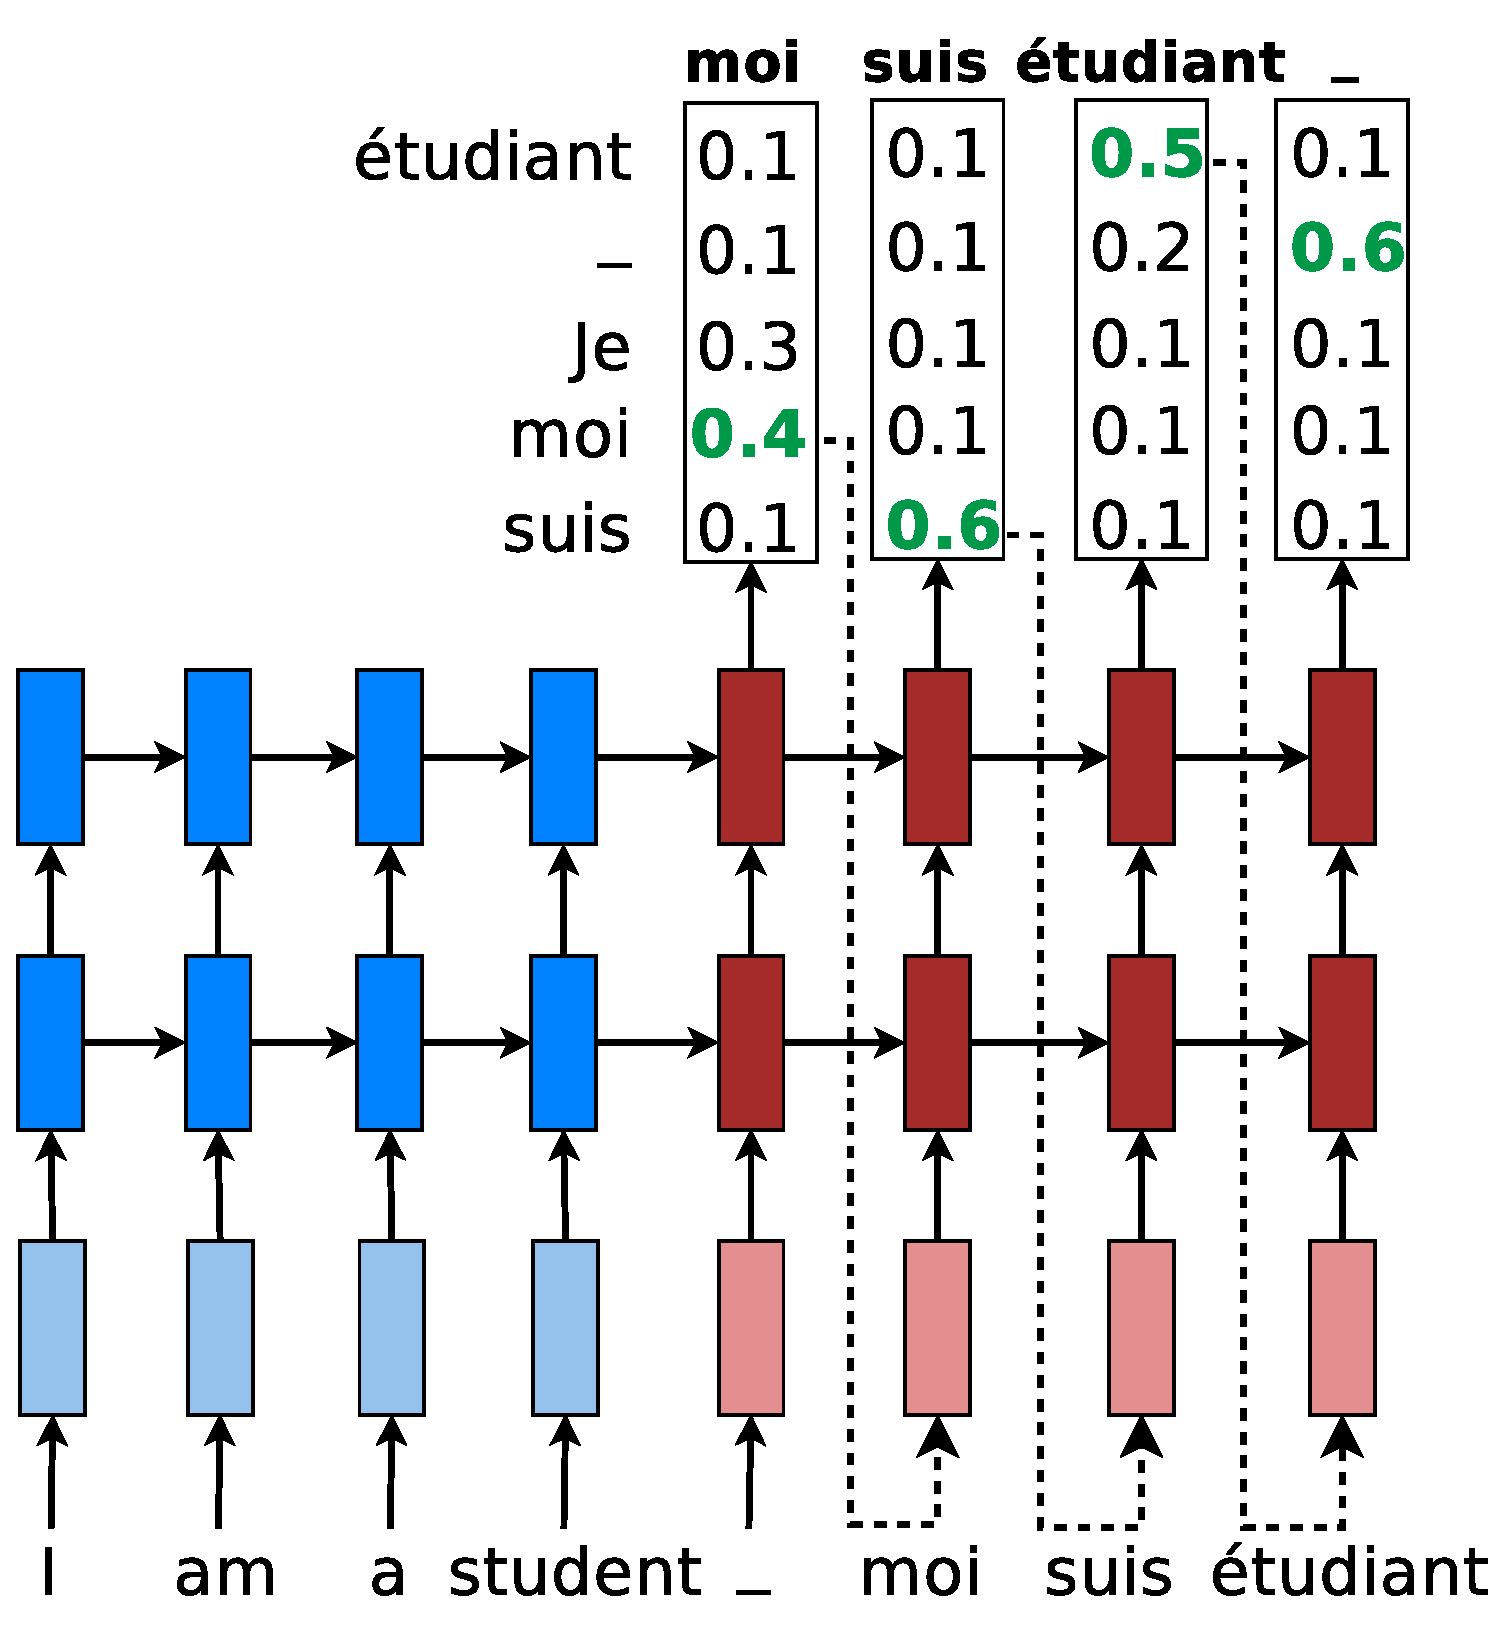
\includegraphics[width=0.6\textwidth, clip=true, trim= 0 0 0
0]{img/nmt_test.eps} % , angle=-90
\caption[Neural machine translation]{{\bf Neural machine translation} -- example of a deep recurrent
architecture proposed by \newcite{sutskever14} for
translating a source sentence \word{I am a student} into a target sentence
\word{Je suis \'{e}tudiant}. Here, \word{\texttt{\_}} marks the end of a sentence.
} 
\label{f:nmt_test}
\end{figure}


%\section{Backward Propagation}
%\subsection{Definitions}
In this section we define some additional notation that will help us to derive the necessary back-propagation equations.

\begin{definition}
Let $U$ and $V$ refer to the $n \times n$ weight matrices corresponding to the following portions of $\MB{T}_{4n \times 2n}$:
\begin{equation}
\MB{T}_{4n \times 2n} = 
\begin{bmatrix}
U_i & V_i \\
U_f  & V_f\\
U_o & V_o\\
U_{\hat{h}} & V_{\hat{h}} \\
\end{bmatrix}
\end{equation}
In particular, we will use the superscript $l$ to denote these matrices used to calculate layer $l$ in Equation (\ref{eqn:LSTMdef1}).
\end{definition}

\begin{definition}
\label{def:z}
For all $l \in \{1,\dots,L\}$ and $t \in \{1,\dots,T\}$, define the \emph{weighted inputs}
\begin{alignat*}{2}
&\zilt = U_i \MB{h_t^{l-1}} + V_i \MB{h_{t-1}^l} \hspace{50pt}
&\zflt = U_f \MB{h_t^{l-1}} + V_f \MB{h_{t-1}^l}\\
&\zolt = U_o \MB{h_t^{l-1}} + V_o \MB{h_{t-1}^l} 
&\zglt = U_{\hat{h}} \MB{h_t^{l-1}} + V_{\hat{h}} \MB{h_{t-1}^l}
\end{alignat*}
so that 
\begin{equation}
\begin{pmatrix}
\ilt \\
\flt \\
\olt \\
\glt
\end{pmatrix}
=
\begin{pmatrix}
\sigm \\
\sigm \\
\sigm \\
\tanh
\end{pmatrix}
\begin{pmatrix}
\zilt \\
\zflt \\
\zolt \\
\zglt
\end{pmatrix}
\end{equation}
where $\sigm$ and $\tanh$ are applied element-wise.
We call $\zilt$ the \emph{weighted input} to the input gate $\ilt$.
\end{definition}

\begin{definition}
Define the \emph{error} of the input, forget, output and input modulation gates at layer $l$ and time $t$ to be
\begin{alignat*}{2}
\dilt &= \fracder{L}{\zilt} \hspace{50pt}
\dflt &&= \fracder{L}{\zflt} \\
\dolt &= \fracder{L}{\zolt} \hspace{50pt}
\dglt &&= \fracder{L}{\zglt} 
\end{alignat*}
where $L$ is the loss function. Note: $\dilt$ is the partial derivative of $L$ with respect to the weighted input $\zilt$, \emph{not} $\ilt$.
\end{definition}

\begin{definition}
Define the \emph{error} of the hidden state and cell and layer $l$ and time $t$ to be
\begin{align}
\dhlt = \fracder{L}{\hlt} \hspace{50pt} \dclt = \fracder{L}{\clt}
\end{align}
where $L$ is the loss function.
\end{definition}

\subsection{Derivations}
In this section we will derive expressions for $\dhlt$, $\dclt$, $\dilt$, $\dflt$, $\dolt$, and $\dglt$ in terms of the $\MB{\delta}$ values for the $(l+1,t)$ and $(l,t+1)$ blocks. 
These expressions will enable us to do back-propagation through time and layers.
If you are not interested in the derivations, skip ahead to Section \ref{subsec:summary} to see the final back-propagation equations.
\begin{lemma}
For $l \in \{1,\dots, L-1\}$ and $t \in \{1, \dots, T-1\}$,
\begin{equation}
\dhlt = 
\begin{bmatrix}
U_i^\top & U_f^\top & U_o^\top & U_{\hat{h}}^\top & V_i^\top & V_f^\top & V_o^\top & V_{\hat{h}}^\top 
\end{bmatrix}
\begin{bmatrix}
\MB{\delta_i^l(t+1)} \\
\MB{\delta_f^l(t+1)} \\
\MB{\delta_o^l(t+1)} \\
\MB{\delta_{\hat{h}}^l(t+1)} \\
\MB{\delta_i^{l+1}(t)} \\
\MB{\delta_f^{l+1}(t)} \\
\MB{\delta_o^{l+1}(t)} \\
\MB{\delta_{\hat{h}}^{l+1}(t)} 
\end{bmatrix}
\end{equation}
where each of the $U$ and $V$ matrices are with respect to layer $l$.
\end{lemma}
Note the left matrix in the multiplication has dimensions $n \times 8n$, the right matrix $8n \times n$, and $\dhlt$ is $n \times 1$.
\begin{proof}
We prove this element-wise. For any $j=1,\dots n$:
\begin{align}
\dhlt_j = \fracder{L}{(\hlt)_j}  & \tag{definition of $\dhlt$} 
\end{align}
Now, because $\hlt$ affects $(z_i,z_f,z_o,z_{\hat{h}})$ for $(l,t+1)$ and $(l+1,t)$, we take the chain rule over these eight variables. Therefore the above equation can be written as
\begin{alignat*}{2}
\sumkn  \Bigg( \quad 
& \fracder{L}{z_i^l(t+1)_k} \fracder{z_i^l(t+1)_k}{(\hlt)_j}    
\quad 
&& + \quad \fracder{L}{z_f^l(t+1)_k} \fracder{z_f^l(t+1)_k}{(\hlt)_j}
\\
+ \quad &  \fracder{L}{z_o^l(t+1)_k} \fracder{z_o^l(t+1)_k}{(\hlt)_j} 
\quad 
&& + \quad \fracder{L}{z_{\hat{h}}^l(t+1)_k} \fracder{z_{\hat{h}}^l(t+1)_k}{(\hlt)_j}
\\
+ \quad  & \fracder{L}{z_i^{l+1}(t)_k} \fracder{z_i^{l+1}(t)_k}{(\hlt)_j} 
\quad 
&& + \quad \fracder{L}{z_f^{l+1}(t)_k} \fracder{z_f^{l+1}(t)_k}{(\hlt)_j} 
\\
+ \quad & \fracder{L}{z_o^{l+1}(t)_k} \fracder{z_o^{l+1}(t)_k}{(\hlt)_j} 
\quad
&& + \quad \fracder{L}{z_{\hat{h}}^{l+1}(t)_k} \fracder{z_{\hat{h}}^{l+1}(t)_k}{(\hlt)_j} 
\quad  \Bigg)
\end{alignat*}
First note that the first of each pair is some $\MB{\delta}$ e.g.
\begin{align}
\fracder{L}{z_i^l(t+1)_k}= \MB{\delta_i^l(t+1)} \tag{by definition}
\end{align}
The second of each pair can be evaluated like so: 
\begin{align}
\fracder{z_i^l(t+1)_k}{(\hlt)_j} &= \parfrac{(\hlt)_j} \left( U_i^l \MB{h_{t+1}^l} + V_i^l \hlt \right)_k \tag{definition of $z_i^l(t+1)$} \\
&= \parfrac{(\hlt)_j} \left( \sum_{m=1}^n (V_i^l)_{km} (\hlt)_m \right) \tag{$U_i^l \MB{h_{t+1}^l} $ does not depend on $\hlt$} \\
&= (V_i^l)_{kj} \tag{expression equals 0 except when $m=j$}
\end{align}
so the first of the eight sums can be written as 
\begin{align}
\sumkn \fracder{L}{z_i^l(t+1)_k} \fracder{z_i^l(t+1)_k}{(\hlt)_j} = 
\sumkn  \MB{\delta_i^l(t+1)} (V_i^l)_{kj} =
\left[ (V_i^l)^\top \MB{\delta_i^l(t+1)} \right]_j
\end{align}
Finding similar expressions for the other seven sums, we obtain
\begin{alignat*}{4}
\dhlt \quad = \quad \quad 
&(U_i^l)^\top \delta_i^l(t+1) \quad
&&+ \quad (U_f^l)^\top \delta_f^l(t+1) \quad 
&&+ \quad (U_o^l)^\top \delta_o^l(t+1) \quad
&&+ \quad (U_{\hat{h}}^l)^\top \delta_{\hat{h}}^l(t+1) \\
+ \quad &(V_i^l)^\top \delta_i^{l+1}(t)
&&+ \quad (V_f^l)^\top \delta_f^{l+1}(t)
&&+ \quad (V_o^l)^\top \delta_o^{l+1}(t)
&&+ \quad (V_{\hat{h}}^l)^\top \delta_{\hat{h}}^{l+1}(t)
\end{alignat*}
\end{proof}

\begin{lemma}
For $l \in \{1,\dots, L\}$ and $t \in \{1, \dots, T-1\}$,
\begin{equation}
\dclt = \MB{\delta_c^l(t+1)} \circ f^l_{t+1} + \dhlt \circ \olt \circ \tanh'(\clt)
\end{equation}
\end{lemma}
\begin{proof}
We prove this element-wise. For any $j=1,\dots n$:
\begin{align}
\dclt_j &= \fracder{L}{(\clt)_j} \tag{definition of $\dclt$}\\
&= \sumkn \fracder{L}{(\MB{c_{t+1}^l})_k} \fracder{(\MB{c_{t+1}^l})_k}{(\clt)_j} + \sumkn \fracder{L}{(\hlt)_k} \fracder{(\hlt)_k}{(\clt)_j} \tag{chain rule} 
\end{align}
The second equality follows from the fact that $\clt$ affects $\hlt$ and $\MB{c_{t+1}^l}$.
For the first part of the expression, note that
\begin{align*}
 \fracder{(\MB{c_{t+1}^l})_k}{(\clt)_j}
&= \parfrac{(\clt)_j} \left( \MB{f^l_{t+1}} \circ \MB{c^l_{t}} + \MB{i^l_{t+1}}  \circ \MB{\hat{h}^l_{t+1}}  \right)_k \tag{by definition of $\MB{c_{t+1}^l}$} \\
&= 
\begin{cases} 
\MB{f^l_{t+1}}  &\mbox{if } k=j \\
0 &\mbox{ otherwise.}
\end{cases} 
\end{align*}
For the second part, note that
\begin{align*}
\fracder{(\hlt)_k}{(\clt)_j} 
&= \parfrac{(\clt)_j} \left( \olt \circ \tanh(\clt) \right)_k \tag{by definition of $\hlt$} \\
&= 
\begin{cases} 
(\olt)_j \tanh'(\clt)_j &\mbox{if } k=j \\
0 &\mbox{ otherwise.}
\end{cases} 
\end{align*}
Combining the previous three equations and using the definitions of $\MB{\delta_c^l(t+1)}$ and $\dhlt$, we obtain
\begin{align}
\dclt_j = \MB{\delta_c^l(t+1)}_j (\MB{f^l_{t+1}})_j + \dhlt_j (\olt)_j \tanh'(\clt)_j 
\end{align}
\end{proof}

\begin{lemma}
For $l \in \{1,\dots, L\}$ and $t \in \{1, \dots, T\}$,
\begin{equation}
\dilt = \dclt \circ \sigm'(\zilt) \circ \glt
\end{equation}
\end{lemma}
\begin{proof}
We prove this element-wise. For any $j=1,\dots n$:
\begin{align} 
\dilt_j &= \fracder{L}{\zilt_j} \tag{definition of $\dilt$} \\
&= \sumkn \fracder{L}{(\clt)_k} \fracder{(\clt)_k}{\zilt_j} \tag{chain rule} \\
&= \sumkn \dclt_k \parfrac{\zilt_j} \left( \flt \circ \MB{c^l_{t-1}} + \ilt \circ \glt \right)_k \tag{definition of $\dclt$ and $\clt$} \\
&= \dclt_j \parfrac{\zilt_j} \left( \ilt \circ \glt \right)_j \tag{expression equals 0 except when $k=j$} \\
&= \dclt_j  \sigm'(\zilt)_j  (\glt)_j \tag{definition of $\ilt$ in terms of $\zilt$}
\end{align}
Note that for the second equality we took the chain rule with respect to the elements of $\clt$, because $\ilt$ affects $\clt$.
\end{proof}
\begin{lemma}
For $l \in \{1,\dots, L\}$ and $t \in \{1, \dots, T\}$,
\begin{equation}
\dflt = \dclt \circ \sigm'(\zflt) \circ \MB{c_{t-1}^l}
\end{equation} 
\end{lemma}
\begin{proof}
We prove this element-wise. For any $j=1,\dots n$:
\begin{align} 
\dflt_j &= \fracder{L}{\zflt_j} \tag{definition of $\dflt$} \\
&= \sumkn \fracder{L}{(\clt)_k} \fracder{(\clt)_k}{\zflt_j} \tag{chain rule} \\
&= \sumkn \dclt_k \parfrac{\zflt_j} \left( \flt \circ \MB{c^l_{t-1}} + \ilt \circ \glt \right)_k \tag{definition of $\dclt$ and $\clt$} \\
&= \dclt_j \parfrac{\zflt_j} \left( \flt \circ \MB{c^l_{t-1}} \right)_j \tag{expression equals 0 except when $k=j$} \\
& = \dclt_j \sigm'(\zflt)_j (\MB{c_{t-1}^l})_j \tag{definition of $\flt$ in terms of $\zflt$}
\end{align}
Note that for the second equality we took the chain rule with respect to the elements of $\clt$, because $\flt$ affects $\clt$.
\end{proof}

\begin{lemma}
For $l \in \{1,\dots, L\}$ and $t \in \{1, \dots, T\}$,
\begin{equation}
\dolt = \dhlt  \circ \sigm'(\zolt) \circ \tanh(\clt)
\end{equation} 
\end{lemma}
\begin{proof}
We prove this element-wise. For any $j=1,\dots n$:
\begin{align} 
\dolt_j &= \fracder{L}{\zolt_j} \tag{definition of $\dolt$} \\
&= \sumkn \fracder{L}{(\hlt)_k} \fracder{(\hlt)_k}{\zolt_j} \tag{chain rule} \\
&= \sumkn \dhlt_k \parfrac{\zolt_j} \left( \olt \circ \tanh(\clt) \right)_k \tag{definition of $\dhlt$ and $\hlt$} \\
&= \dhlt_j \parfrac{\zolt_j} \left( \olt \circ \tanh(\clt) \right)_j \tag{expression equals 0 except when $k=j$} \\
&= \dhlt_j \sigm'(\zolt)_j \tanh(\clt)_j \tag{definition of $\olt$ in terms of $\zolt$}
\end{align}
Note that for the second equality we took the chain rule with respect to the elements of $\hlt$, because $\olt$ affects $\hlt$.
\end{proof}

\begin{lemma}
For $l \in \{1,\dots, L\}$ and $t \in \{1, \dots, T\}$,
\begin{equation}
\dglt = \dclt \circ \ilt \circ \tanh'(\zglt)
\end{equation} 
\end{lemma}
\begin{proof}
We prove this element-wise. For any $j=1,\dots n$:
\begin{align} 
\dglt_j &= \fracder{L}{\zglt_j} \tag{definition of $\dglt$} \\
&= \sumkn \fracder{L}{(\clt)_k} \fracder{(\clt)_k}{\zglt_j} \tag{chain rule} \\
&= \sumkn \dclt_k \parfrac{\zglt_j} \left( \flt \circ \MB{c^l_{t-1}} + \ilt \circ \glt \right)_k \tag{definition of $\dclt$ and $\clt$} \\
&= \dclt_j \parfrac{\zglt_j} \left(\ilt \circ \glt  \right)_j \tag{expression equals 0 except when $k=j$} \\
&= \dclt_j (\ilt)_j \tanh'(\zglt)_j \tag{definition of $\glt$ in terms of $\zglt$}
\end{align}
Note that for the second equality we took the chain rule with respect to the elements of $\clt$, because $\glt$ affects $\clt$.
\end{proof}


\begin{lemma}
\label{lem:weight_derivs}
For all $l \in \{1,\dots,L\}$,
\begin{align*}
\fracder{L}{U_i^l} &= \sum_{t=1}^T (\MB{h_t^{l-1}}) (\dilt)^\top 
&\fracder{L}{V_i^l} &= \sum_{t=1}^T (\MB{h_{t-1}^l}) (\dilt)^\top \\
\fracder{L}{U_f^l} &= \sum_{t=1}^T (\MB{h_t^{l-1}}) (\dflt)^\top 
&\fracder{L}{V_f^l} &= \sum_{t=1}^T (\MB{h_{t-1}^l}) (\dflt)^\top \\
\fracder{L}{U_o^l} &= \sum_{t=1}^T (\MB{h_t^{l-1}}) (\dolt)^\top 
&\fracder{L}{V_o^l} &= \sum_{t=1}^T (\MB{h_{t-1}^l}) (\dolt)^\top \\
\fracder{L}{U_{\hat{h}}^l} &= \sum_{t=1}^T (\MB{h_t^{l-1}}) (\dglt)^\top 
&\fracder{L}{V_{\hat{h}}^l} &= \sum_{t=1}^T (\MB{h_{t-1}^l}) (\dglt)^\top 
\end{align*}
\end{lemma}
\begin{proof}
We will prove the identities for the input gate $i$ only; the proofs for $f$, $o$ and $\hat{h}$ are identical.
First recall Definition \ref{def:z} for the weighted input:
\begin{equation*}
\zilt = U_i \MB{h_t^{l-1}} + V_i \MB{h_{t-1}^l} 
\end{equation*}
Now, for any $j,k \in \{1,\dots,n\}$, consider the effect of $(U_i^l)_{jk}$. It maps from the $k$th element of $\MB{h_t^{l-1}}$ to the $j$th element of $\zilt$, for all $t$. Therefore applying the chain rule we obtain
\begin{align}
\fracder{L}{(U_i^l)_{jk}} &= \sum_{t=1}^T \fracder{L}{\zilt_j} \fracder{\zilt_j}{(U_i^l)_{jk}} \tag{chain rule} \\
&= \sum_{t=1}^T \dilt_j (\MB{h_t^{l-1}})_k \tag{definition of $\dilt$ and $\zilt$}
\end{align}
Therefore
\begin{align}
\fracder{L}{(U_i^l)} = \sum_{t=1}^T  (\MB{h_t^{l-1}}) (\dilt)^\top
\end{align}
The expression for $\partial L / \partial V_i^l$ is derived similarly, by noting that $(V_i^l)_{jk}$ maps from the $k$th element of $\MB{h_{t-1}^l}$ to the $j$th element of $\zilt$.
\end{proof}

\begin{corollary}
For all $l \in \{1,\dots,L\}$,
\begin{align}
\begin{bmatrix}
\partial L / \partial U_i^l & \partial L / \partial V_i^l \\
\partial L / \partial U_f^l & \partial L / \partial V_f^l \\
\partial L / \partial U_o^l & \partial L / \partial V_o^l \\
\partial L / \partial U_{\hat{h}}^l & \partial L / \partial V_{\hat{h}}^l
\end{bmatrix}
= \sum_{t=1}^T 
\begin{bmatrix}
\dilt \\
\dflt \\
\dolt \\
\dglt
\end{bmatrix}
\begin{bmatrix}
\MB{h_t^{l-1}} & \MB{h_{t-1}^l}
\end{bmatrix}
\end{align}
\end{corollary}
\begin{proof}
This is simply a rearrangement of Lemma \ref{lem:weight_derivs}.
\end{proof}




\subsection{Summary}
\label{subsec:summary}
Now we have derived all the necessary equations, we have an algorithm to calculate the necessary error values for each LSTM block, and thus calculate the derivative of the loss function with respect to our various weights.

For $l \in \{1,\dots,L-1\}$ and $t \in \{1,\dots,T\}$, we calculate $\dhlt$ as follows: 
\begin{align*}
\dhlt &= 
\begin{bmatrix}
U_i^\top & U_f^\top & U_o^\top & U_{\hat{h}}^\top & V_i^\top & V_f^\top & V_o^\top & V_{\hat{h}}^\top 
\end{bmatrix}
\begin{bmatrix}
\MB{\delta_i^l(t+1)} \\
\MB{\delta_f^l(t+1)} \\
\MB{\delta_o^l(t+1)} \\
\MB{\delta_{\hat{h}}^l(t+1)} \\
\MB{\delta_i^{l+1}(t)} \\
\MB{\delta_f^{l+1}(t)} \\
\MB{\delta_o^{l+1}(t)} \\
\MB{\delta_{\hat{h}}^{l+1}(t)} 
\end{bmatrix} \\
\dclt &= \MB{\delta_c^l(t+1)} \circ f^l_{t+1} + \dhlt \circ \olt \circ \tanh'(\clt)\\
\dilt &= \dclt \circ \sigm'(\zilt) \circ \glt \\
\dolt &= \dhlt  \circ \sigm'(\zolt) \circ \tanh(\clt) \\
\dflt &= \dclt \circ \sigm'(\zflt) \circ \MB{c_{t-1}^l} \\
\dglt &= \dclt \circ \ilt \circ \tanh'(\zglt)
\end{align*}
Note: if $t=T$ then we take $\MB{\delta^l(t+1)}$ to be zero for $\MB{i}$, $\MB{f}$, $\MB{o}$, $\MB{\hat{h}}$ and $\MB{c}$. 
\todo{if $l=L$ how do we calculate $\dhlt$?}

Once we have calculated the above error values for all $l$ and $t$, we can calculate the derivative of the loss function with respect to our various weights. In particular, for $l \in \{1,\dots,L\}$:
\begin{align*}
\begin{bmatrix}
\partial L / \partial U_i^l & \partial L / \partial V_i^l \\
\partial L / \partial U_f^l & \partial L / \partial V_f^l \\
\partial L / \partial U_o^l & \partial L / \partial V_o^l \\
\partial L / \partial U_{\hat{h}}^l & \partial L / \partial V_{\hat{h}}^l
\end{bmatrix}
= \sum_{t=1}^T 
\begin{bmatrix}
\dilt \\
\dflt \\
\dolt \\
\dglt
\end{bmatrix}
\begin{bmatrix}
\MB{h_t^{l-1}} & \MB{h_{t-1}^l}
\end{bmatrix}
\end{align*}
We then use these derivatives to apply gradient descent to $U^l$ and $V^l$.




%\section{Other Recurrent Units}
%Different recurrent units:
%
%GRU \cite{cho14}
%\begin{align}
%\begin{pmatrix}
%\MB{z_t} \\
%\MB{r_t} \\
%\end{pmatrix}
%&= 
%\begin{pmatrix}
%\sigm \\
%\sigm \\
%\end{pmatrix}
%\MB{T}_{2n \times 2n}
%\begin{bmatrix}
%  \MB{x_t} \\
%  \MB{h_{t-1}}
% \end{bmatrix} \\ 
%\MB{\hat{h}_t} &= \tanh(\MB{W} \MB{x_t} + \MB{r_t} \circ \MB{U}\MB{h_{t-1}}) \\
%\MB{h_t} &= \MB{z_t} \circ \MB{h_{t-1}} + (1-\MB{z_t}) \circ \MB{\hat{h}_t}
%\end{align}
%
%My unit (maybe we should try to implement this!)
%\begin{align}
%\begin{pmatrix}
%\MB{i_t} \\
%\MB{f_t} \\
%\MB{\hat{h}_t} \\
%\end{pmatrix}
%&= 
%\begin{pmatrix}
%\sigm \\
%\sigm \\
%\tanh
%\end{pmatrix}
%\MB{T}_{3n \times 2n}
%\begin{bmatrix}
%  \MB{x_t} \\
%  \MB{h_{t-1}}
% \end{bmatrix} \\
%\MB{h_t} &= \MB{f_t} \circ \MB{h_{t-1}} + \MB{i_t} \circ \MB{\hat{h}_t}
%\end{align}

%\subsection{Attention}
%Content-based
%\begin{align}
%\al = Attend(\hd{t-1}, \MB{\bar{h}}_{1 \ldots S}) 
%\end{align}
%
%Location-based
%\begin{align}
%\al = Attend(\hd{t-1}, \MB{a}_{t-1})
%\end{align}
%
%Hybrid
%\begin{align}
%\al = Attend(\hd{t-1}, \MB{a}_{t-1}, \MB{\bar{h}}_{1 \ldots S})
%\end{align}

%The target word with the highest score is selected as the output translation.

%\noindent {\bf Attention Mechanism} -- 
%The early NMT approaches \cite{sutskever14,cho14}, which we have described above, use only the last encoder state
% to initialize the decoder, i.e., setting the input representation $\MB{s}$ in
% \eq{e:s2s} to $[\hb{n}]$. Recently, \newcite{bog15} propose an {\it attention
% mechanism}, a form of random access memory for NMT to 
%cope with long input sequences.
%\newcite{luong15attn} further extend the attention mechanism to different
%scoring functions, used to compare source and target
%hidden states, as well as different
%strategies to place the attention.
%In all our models, we utilize the {\it global} attention mechanism and the {\it
%bilinear form} for the attention scoring function similar to 
%\cite{luong15attn}.
%
%\begin{figure}
%\centering
%%\psgrid
%\rput(4.3,6.5){$\tgt{t}$}
%\rput(1.4,5.6){$\mem{t}$}
%\rput(0.8,3.1){$\hb{1}$}
%\rput(2.9,3.1){$\hb{n}$}
%\rput(4.9,3.1){$\hid{t}$}
%\rput(4.9,6.0){$\hs$}
%%\rput(4.0,3.8){$\hd{t-1}$}
%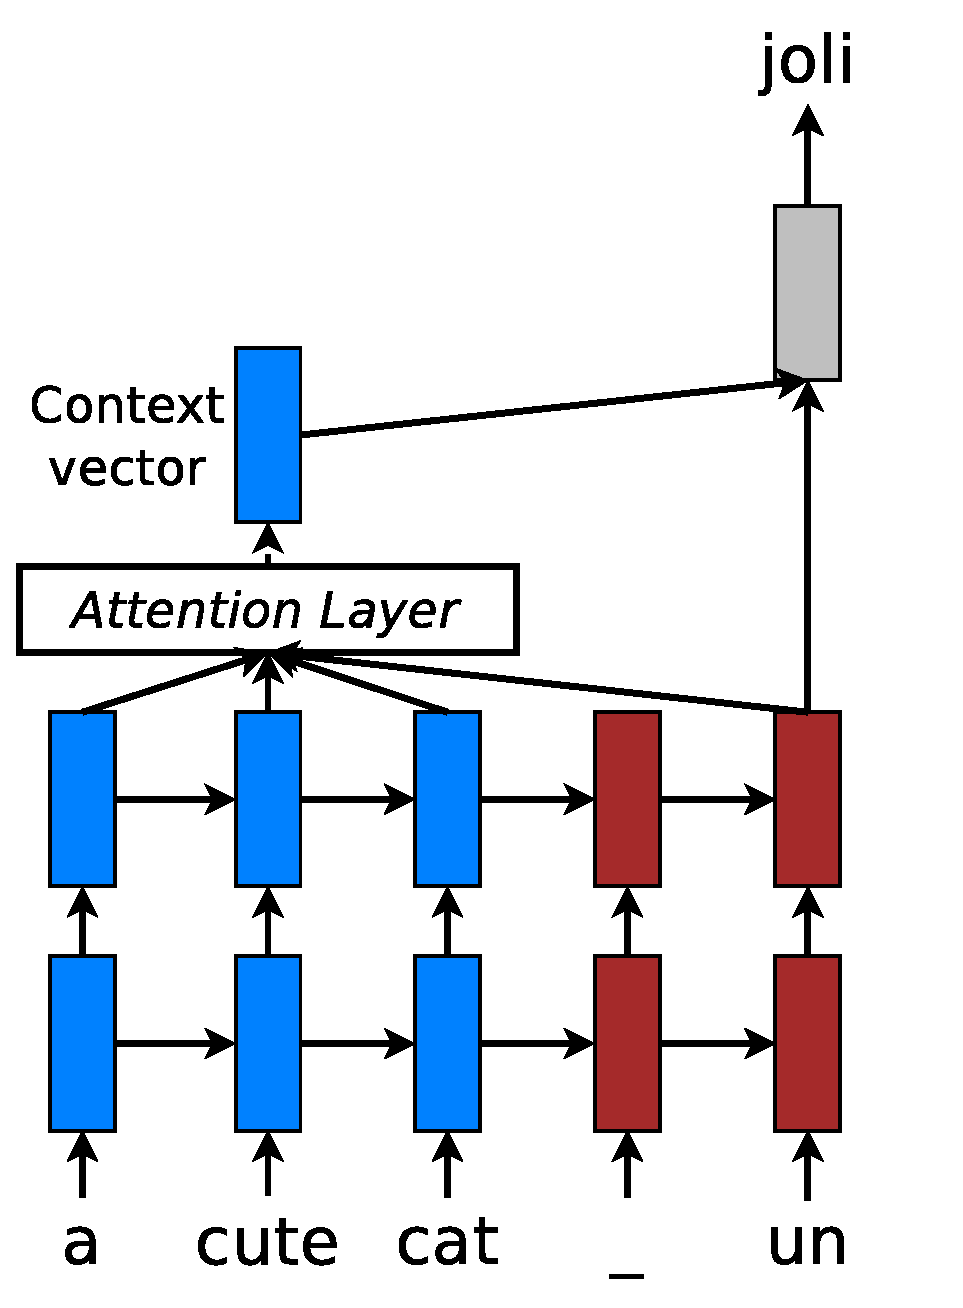
\includegraphics[width=0.33\textwidth, clip=true, trim= 0 0 0 0]{img/attn.eps} % , angle=-90
%\caption{{\bf Attention mechanism}.
%} 
%\label{f:attn}
%\end{figure}
%
%Specifically, we set $\MB{s}$ in \eq{e:s2s} to
%the set of source hidden states at the top layer, $[\hb{1}, \dots, \hb{n}]$. 
%As illustrated in Figure~\ref{f:attn}, the attention mechanism consists of two stages: (a) {\it
%context vector} -- the current hidden state $\hid{t}$ is compared with
%individual source hidden states in $\MB{s}$ to learn an alignment vector, which
%is then used to compute the context vector $\co$ as a weighted average of
%$\MB{s}$; and (b) {\it
%attentional hidden state} -- the context vector $\co$ is then used to derive a
%new attentional hidden state:
%\begin{equation}
%\hs = \tanh(\W{}[\co; \hi])
%\label{e:hs}
%\end{equation} 
%The attentional vector $\hs$ then replaces $\hid{t}$ in \eq{e:softmax} in
%predicting the next word.

%\newcite{kal13} used an RNN with the vanilla RNN unit for the decoder and a
%convolutional neural network for encoding the source. On
%the other hand, \newcite{sutskever14} and our work built deep RNNs with the LSTM unit
%for both the encoder and the decoder. \newcite{cho14},  
%\newcite{bog15}, inter alia, adopted an
%LSTM-inspired hidden unit, the gated recurrent unit (GRU), and used bidirectional
%RNNs for the encoder.

%In more detail, considering the top recurrent layer in a deep RNN architecture, one can compute the probability of decoding each target word $y_j$ as:
%\begin{equation}
%p\left(\tgt{j}|\tgt{<j},\src{},\MB{s}\right) = \softmax\paren{\hid{j}}
%\end{equation}
%with $\hid{j}$ being the current target hidden state computed as:
%\begin{equation}
%\label{e:rnn}
%\hid{j} = f(\hid{j-1}, \tgt{j-1}, \MB{s})
%\end{equation}
%Here, $f$ derives the current state given the previous state
%$\hid{j-1}$, the
%current input (often the previous word $\tgt{t-1}$), and optionally, the source
%representation $\MB{s}$.
%$f$ can be a vanilla RNN unit, a GRU, or an LSTM. 
%The early NMT approach  \cite{kal13,sutskever14,cho14,luong15} uses the last source hidden state
%$\MB{s}=\hb{n}$ once to initialize the decoder hidden state and sets $\MB{s}=[\text{ }]$ in
%\eq{e:rnn}.

